\chapter{Related Work and Design Space}
\label{chap:design_space}

The previous chapter established what graphs are, how they are accessed, and how they are stored.
This chapter surveys the systems that have been built to manage and process graph data, and organizes them into a taxonomy based on three classification features: whether a system operates on property graphs or structural graphs, whether it handles a static snapshot or a dynamic, evolving graph, and whether it provides transactional guarantees for mutations.
We discuss representative systems in each category, highlighting what each provides and what it lacks, and conclude with a distillation of the design space that positions FlexoGraph as a general-purpose system spanning the entire grid.


\section{Property Graphs vs. Structural Graphs}
\label{design:property_vs_structural}
Our overarching characterization of the design space is defined by two features: whether the system manages property graphs or structural graphs and whether the graphs under management are static or dynamic.
Recall that a structural graph results from selections and projections on the labels and properties of an underlying property graph~\cite{RodriguezNeubauer2010}.
One might select edges of a certain type to form a structural graph, for instance, a structural graph of follower relationships in a social network.
The structural graph so constructed ``is homogeneous, composed simply of vertices, edges and, possibly, a weight attached to their elements''~\cite{teseo2021deLeo}.
The structural graph is a useful abstraction for many graph algorithms and queries. It provides a simple graph model that can be used to reason about the graph's structure.
For instance, the structural graph can be used to compute the connectivity of the graph or to compute the influence of a node in the graph.

We assume that the property graph represents ground truth and that the structural graph is derived from the property graph.
A structural graph can be materialized as needed or periodically, as is done at Facebook~\cite{curtiss2013unicorn}.
These materialized structural graphs are essentially snapshots of the property graph at a certain point in time.
We describe these \emph{static structural graphs} in more detail in~\autoref{design:static_structural}.

In contrast, the property graph changes over time.
Since the property graph is the ground truth, it is important to keep the structural graph up-to-date with the property graph.
This can be done by periodically recomputing the structural graph or incrementally updating it as the property graph changes.
This leads to the concept of \emph{dynamic structural graphs}, which are updated as the property graph changes.
We describe dynamic structural graphs in more detail in~\autoref{design:dynamic_structural}.

\project{} stores both the property graph and its derived structural representations in the same transactional \wt{} store.
Structural graphs are not separate materialized snapshots that must be rebuilt or shipped to a different engine; they are persistent layouts maintained alongside the property data.
Switching between property queries and structural analytics therefore requires no data movement.


\section{Static Graph Processing Systems}
\label{design:static_structural}

Static structural graphs have been the main focus of graph processing systems research for over a decade (~\cite{malewicz2010pregel,gonzalez2014graphx, zhu2016gemini, xing2015petuum, low2012distributed,gonzalez2012powergraph, powerlyra2019,shun2013ligra, nguyen2013lightweight, zhu2016gemini, graphmat, lakhotia2020gpop, beamer2015gap, kim2022blaze, ai2018clip,zheng2015flashgraph}).
These graphs are primarily used for analytics and graph mining tasks focusing on uncovering statistical properties and discovering patterns.
The static nature of these graphs implies that there is no consistency requirement between different snapshots that these systems are designed to process.
Each snapshot is produced through a batch \ac{ETL} process and is (often) processed independently of other snapshots.
On the other hand, in a graph database, the graph is materialized from the property graph, and that is the "extract" step when creating structural graphs.

Once the static GPS has a snapshot to process, it must first \emph{preprocess} the graph to construct the data structures needed to execute the graph algorithms.
The preprocessing step is often the most time-consuming in the graph processing pipeline.
The preprocessing step involves reading a graph in a data exchange format (often a CSV file) and using that to construct and populate a suitable data structure to hold the graph.
This requires a pass over the graph and can take significantly longer to finish than the analytics task itself (for example, GraphChi takes longer to preprocess the graph than it takes to run Triangle Counting or PageRank).

If the graph data structures obtained after the preprocessing are small enough, they can be stored and processed in memory.
Graph processing systems designed for shared-memory, multi-core machines are usually optimized for in-memory processing.
Several systems have been optimized for this design point, for example, Gemini~\cite{zhu2016gemini}, GraphMat~\cite{graphmat}, Ligra~\cite{shun2013ligra}, Galois~\cite{pingali2011tao}, GPOP~\cite{lakhotia2020gpop}, and GraphLab~\cite{low2012distributed}.
The GAP Benchmark Suite (GAPBS)~\cite{beamer2015gap} provides optimized reference implementations of common analytics kernels on a CSR representation; FlexoGraph adapts these kernels to use its API for a fair comparison.
Ligra~\cite{shun2013ligra} introduces direction-optimizing traversal that switches between sparse and dense modes based on frontier size.
Galois~\cite{nguyen2013lightweight} generalizes graph computation with priority-driven scheduling for irregular parallelism.
Gemini~\cite{zhu2016gemini} uses chunk-based partitioning with locality-aware execution.

If the graph structures are too large to fit in memory on a single machine, they are partitioned across multiple machines.
Examples of distributed graph processing systems include GraphX~\cite{gonzalez2014graphx}, Pregel~\cite{malewicz2010pregel}, PowerGraph~\cite{gonzalez2012powergraph}, Distributed GraphLab~\cite{low2012distributed}, and PowerLyra~\cite{powerlyra2019}.
For the purpose of our taxonomy, we collectively refer to shared-memory multi-core systems and distributed (in-memory) systems as \textbf{in-memory graph} processing systems.

Over time, researchers noticed that the communication overheads in distributed graph processing systems were high, leading them to underperform when compared to single-threaded systems running on a commodity laptop~\cite{mcsherry2015scalability}.
The need to build systems that can scale to large graphs that do not fit in RAM on a single machine, coupled with the underperformance of distributed graph processing systems, led to the development of out-of-core systems.
These systems cache the most frequently accessed data structures in memory and spill the rest to disk; we call them \textbf{out-of-core graph} processing systems.
The on-disk data layout is designed to leverage sequential access to edge data to minimize I/O overheads.
Most systems achieve this by some form of edge-list partitioning such that the neighbors (either in- or out-neighbors) of a vertex are stored contiguously on disk.
GraphChi~\cite{kyrola2012graphchi} partitions edges into shards processed via Parallel Sliding Windows;
X-Stream~\cite{roy2013x} streams unordered edge lists through memory in a scatter-gather model;
Blaze~\cite{kim2022blaze} targets NVMe SSDs with partition-centric processing and I/O scheduling optimized for high device parallelism.
Other out-of-core systems include GridGraph~\cite{zhu2015gridgraph}, V-part~\cite{elyasi2019large}, Wonderland~\cite{zhang2018wonderland}, CLIP~\cite{ai2018clip}, and FlashGraph~\cite{zheng2015flashgraph}.

All static systems, whether in-memory or out-of-core, require an offline preprocessing step to build their layout and are batch-only, supporting no mutations during processing.
FlexoGraph operates directly on its persistent representation, eliminating the preprocessing step entirely; we include preprocessing time in all comparisons to capture this advantage.
FlexoGraph relies on WiredTiger's buffer pool to spill to secondary storage, achieving competitive out-of-core performance without a dedicated I/O framework.
These two classes of graph processing systems constitute the \textit{third classification feature} of our design space of graph data management systems.

\section{Dynamic Graph Processing Systems}
\label{design:dynamic_structural}
Structural graphs are derived from property graphs, and since the property graph is dynamic, the structural graph must be updated as the property graph changes; this leads to the concept of dynamic structural graphs.
The dynamic nature of these graphs requires some form of consistency.
The structural graph must be updated in a manner consistent with the updates applied to the property graph while simultaneously ensuring that concurrent queries on the structural graph are not affected by the updates.

A dynamic system can apply updates to the structural graph directly without considering ongoing queries.
When such a system applies an update (adding a new edge, for instance), it applies the update to the live graph data structure without creating any new versions.
Any ongoing queries running on the graph data structure will see the update immediately, which can lead to incorrect or inconsistent results, query failures, or delayed convergence of iterative algorithms.
STINGER~\cite{stinger2012ediger} is an example of such a system that allows for fast updates to the graph data structure but does not provide any consistency guarantees.

A more sophisticated approach is to construct a new version of the structural graph as the updates arrive.
Each update to the graph has an associated timestamp, and a system uses these timestamps to construct a versioned graph.
The system can then provide a consistent view of the graph at a certain point in time by selecting the appropriate versions of the graph elements.
Examples of systems that use this approach include GraphOne~\cite{graphone2019kumar}, LLAMA~\cite{llama}, and ASPEN~\cite{10.1145/3314221.3314598}.

Another approach is to batch updates and apply them together to maintain a single incremental view of the graph.
The interesting challenge in these systems is to make sure that any in-progress computations are not affected by the updates and can continue to make progress with the new data.
These systems are designed to use incremental algorithms that can minimize redundant computation by reusing results that have been computed before the graph structure mutates.
GraphBolt~\cite{mariappan2019graphbolt}, for instance, uses ``dependency-driven incremental processing, in which it first tracks dependencies to capture how intermediate values are computed and then uses this information to incrementally propagate the impact of change across intermediate values.''
Kickstarter~\cite{vora2017kickstarter}, GraphIn~\cite{sengupta2016graphin}, and Tornado~\cite{shi2016tornado} are other systems that use a similar approach.

The most sophisticated approach to handling dynamic graphs is to provide a transactional interface to the user.
Transactions help a system provide some or all of the ACID guarantees in the presence of updates.
Good examples of transactional dynamic graph processing systems include LiveGraph~\cite{zhu2019livegraph}, Sortledton~\cite{sortledton2022Fuchs}, and Teseo~\cite{teseo2021deLeo}.
Teseo organizes edges in a fat-tree of dense pages that are periodically rebalanced for locality.
GraphOne~\cite{graphone2019kumar} uses an append-only edge log paired with an adjacency array, with blind-write semantics and no conflict detection.
LiveGraph maintains a transactional edge log with mmap-backed adjacency-list snapshots and is the closest system to FlexoGraph in scope.
Sortledton is an in-memory system that provides a fully transactional adjacency-list based graph data structure; GTX~\cite{libinzhou2025GTX} offers similar capabilities.
Sortledton and GTX achieve higher raw throughput than Teseo on several benchmarks, but we compare primarily against Teseo because it is a more established baseline and, like \project{}, uses a tree-based index structure.
We compare against these systems using the GFE driver~\cite{teseo2021deLeo} for fair, reproducible benchmarking.
FlexoGraph shows that a persistent, B-tree-backed database can deliver competitive throughput without sacrificing ACID semantics or crash recovery.

The consistency model used by these systems falls along a spectrum (the left-right axis in the right branch of~\autoref{fig:design_space} points in the direction of diminishing consistency guarantees).
To construct a taxonomy, we use a simple binary feature to characterize this consistency axis: does the system support transactions or not?
Graph Databases and a few systems (LiveGraph, Teseo, and Sortledton) support transactions which allow for fine-grained guarantees for individual updates to the graph; the remaining systems provide some form of batch-dynamism: isolation is coarse grained and therefore weaker.

\project{} addresses the consistency spectrum differently from all four categories.
It provides full ACID transactions via \wt{}'s MVCC for point queries and mutations, while analytics run against a pinned named checkpoint---a reconciled, consistent snapshot of the B-tree.
Running analytics at a checkpoint rather than on the live table avoids the cost of reading through un-reconciled writes in the cache under write-heavy workloads.
This design gives \project{} transactional isolation without the blind-write semantics of GraphOne, the batch-only granularity of GraphBolt, or the lack of consistency guarantees of STINGER, while avoiding the performance penalty of snapshot-isolated reads on a heavily mutated live table.

The static structural graph processing systems can be seen in the bottom left corner of the design space in~\autoref{fig:design_space}, while the dynamic structural graph processing systems occupy the bottom right.
\autoref{fig:design_space} shows the memory-based/out-of-core axis as a gradient, where the out-of-core systems are shown in yellow shades, while the in-memory systems are shades of red.
This classification is based on the observation that most out-of-core systems can act like an in-memory system when the graph is small.

\begin{figure}[h]
    \centering
    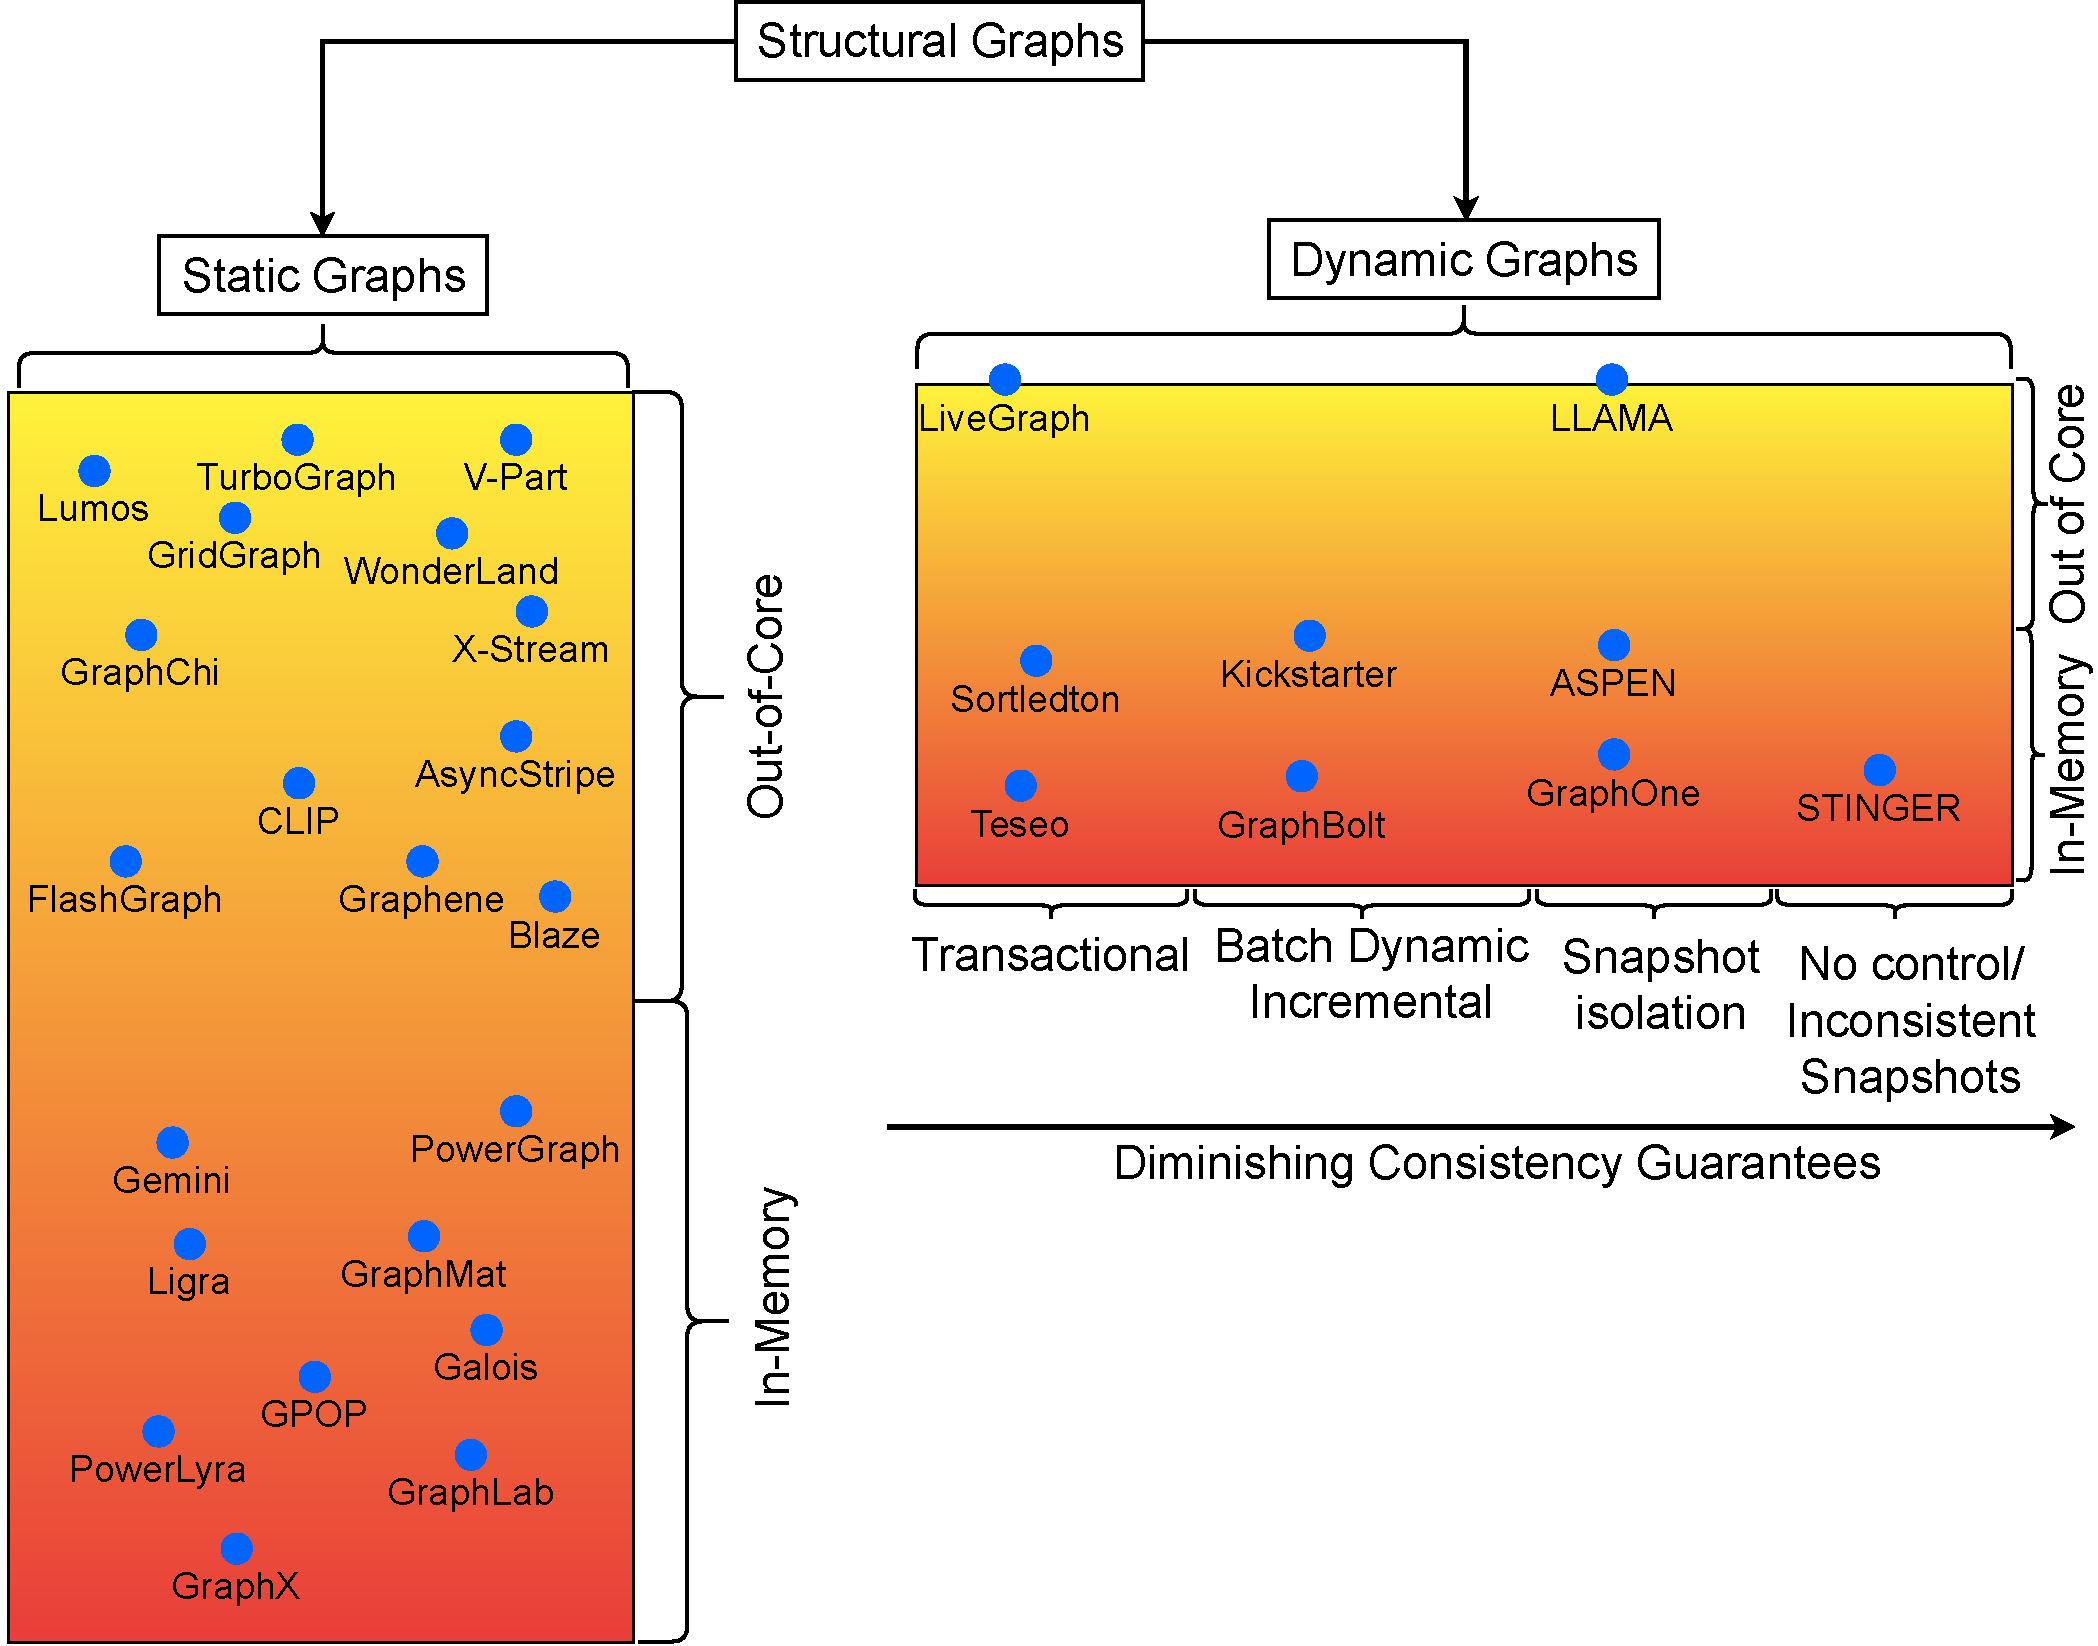
\includegraphics[width=0.8\textwidth]{fig/background/final_taxonomy_struc.pdf}
    \caption{Design Space of Graph Data Management Systems}
    \label{fig:design_space}
\end{figure}

\section{Programming and Computation Models}
\label{design:programming_vs_computation}
The design space of graph processing systems can be further subdivided based on the programming and computation models for which they are designed.
Several survey papers~\cite{mccune2015tlavSurvey, Heidari:2018:SGP:3212709.3199523} discuss this classification in far more detail; we present an overview here and then explain how the choice of programming model motivates \project{}'s dual-representation design.

\subsection{Computation Models}
\label{design:comp_models}

Graph processing systems are designed to execute iterative algorithms in distinct phases.
A \textbf{Computation Model} defines these phases and the sequence in which they must be run.
The user typically writes the algorithm in terms of these phases, and the system executes the algorithm by running these phases in sequence.
The computation model is independent of the system's scheduling model, which determines which vertices are selected for computation (i.e., remain active) in each phase.

The most well-known computation model is the \textbf{Bulk Synchronous Parallel (BSP)} model~\cite{valiant1990bridging}.
This model is based on the idea of supersteps, where the computation is divided into a sequence of supersteps, each consisting of a computation phase and a communication phase.
The computation phase is where a user-defined function executes on each of the graph's vertices, and the communication phase is where the vertices exchange messages.
The BSP model \textit{pushes} updates to the vertices at the end of each superstep and applies these updates to the graph at the beginning of the next superstep.
Examples of systems that use this model include Pregel~\cite{malewicz2010pregel} and Giraph~\cite{giraph}.

The \textbf{Asynchronous} model is a computation model where the computation is not divided into supersteps.
In the Asynchronous model, vertices make updates visible immediately; there is no clear delineation between supersteps.
These systems need a consistency model for updating the edges and vertices.
Examples of these systems include GRACE, ASPIRE, Giraph Unchained, CoRAL, and GraphChi~\cite{kyrola2012graphchi}.

\textbf{Gather-Apply-Scatter} (GAS) is a more general computation model that can describe both BSP and Asynchronous models.
The GAS model consists of three phases: Gathering updates by \emph{pulling} them from neighbors, computing and applying the updates, and \emph{pushing} the updates to the neighbors.
Systems built using this model include GraphLab~\cite{low2012distributed}, PowerGraph~\cite{gonzalez2012powergraph}, and GraphX~\cite{gonzalez2014graphx}.

\subsection{Programming Models}
\label{design:prog_models}

Orthogonal to the computation model is the \textbf{Programming Model} used by the system.
The programming model defines the interface provided to the user to write graph algorithms and, therefore, defines the unit of computation in a system.

The most common programming model is the \textbf{Vertex-Centric} model, where the user writes a function that operates on each vertex of the graph.
Each vertex program can read the state of the vertex and its neighbors and update the state of the vertex.
The user provides a \texttt{compute()} function, a \texttt{get\_value()} function to read the neighbors' state, and a \texttt{update\_state()} function to update the state of the vertex.

The \textbf{Edge-Centric} model is another programming model where the user writes a function that operates on each edge of the graph.
Edge-centric processing was introduced by X-Stream~\cite{roy2013x}, which observed that organizing computation per-edge converts random access to graph structure into sequential streaming---an access pattern that is efficient across all levels of the storage hierarchy.
Edge-centric models propagate changes by updating the state of the edge and the state of the vertices connected by the edge.
The user provides an \texttt{edge\_scatter(e)} function that sends an update over the edge $e$, an \texttt{edge\_gather(e)} function that reads the update from the edge $e$, and an \texttt{apply(e)} function that applies the update to the edge's destination vertex $e.dest$.

The \textbf{Partition Centric} model is a third programming model where the user writes a function executed on each graph partition.
This model is used by systems that are expressly designed to reduce cross-partition communication overhead in a distributed graph processing system.

The programming and computation models are orthogonal, and a system can use any combination.
The design space of static graph processing systems can be split based on these two axes, as shown in~\autoref{fig:static_ec_vc}.

\begin{figure}
    \centering
    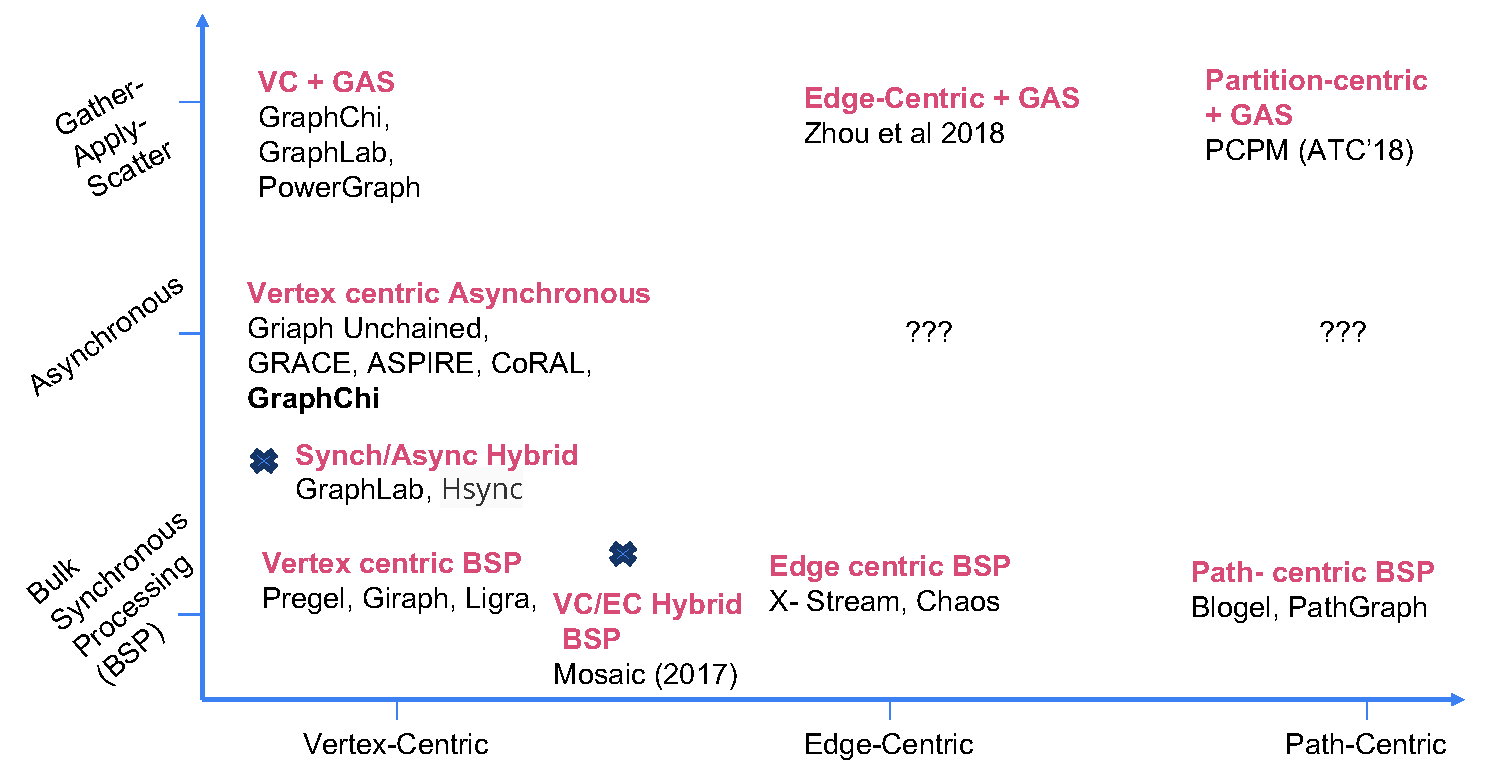
\includegraphics[width=0.8\textwidth]{fig/background/vc_ec.pdf}
    \caption{Splitting the space of static graph processing systems based on the programming model (x-axis) and the computation model (y-axis). The systems marked with a blue X are hybrid: Mosaic~\cite{maass2017mosaic} is a hybrid vertex-centric/edge-centric system, while GraphLab~\cite{low2014graphlab} and Hsync~\cite{Xie2015Hsync} are hybrid in their computation model and switch between synchronous and asynchronous modes of computation.}
    \label{fig:static_ec_vc}
\end{figure}

As the figure shows, the Vertex-Centric model is the most common programming model used by graph processing systems, and there are some combinations of programming and computation models that are not used by any system.
The dominance of vertex-centric systems in the figure is not accidental---it reflects a deep coupling between physical representation and programming model that we explore next.

\subsection{Representation and Computation Model Pairing}
\label{design:rep_comp_pairing}

Each programming model implies a dominant access pattern, and the physical representation of the graph determines how efficiently that pattern executes.
Understanding this coupling is important for \project{}'s design, because it explains why we provide two structural representations and how each representation naturally pairs with a different programming model.

Vertex-centric systems such as Ligra, Galois, and GAPBS store the graph in packed adjacency lists or CSR arrays.
In these layouts, a single read retrieves all neighbors of a vertex, so the cost of a full graph scan is proportional to the number of vertices, not edges.
This is highly efficient for read-heavy analytics: an algorithm like PageRank iterates over each vertex, reads its neighbor list in one operation, and computes a local update.
However, this packing comes at a cost for mutations.
Inserting or deleting a single edge requires a read-modify-write of the packed buffer---the system must read the entire neighbor list, modify it, and write it back---which is expensive for high-degree vertices and creates a serialization bottleneck under concurrent mutation.

Edge-centric systems such as X-Stream and Chaos~\cite{roy2015chaos} take the opposite approach: they store edges as individual records that are streamed sequentially.
Each edge is independently accessible, so edge insertions and deletions are simple appends or point deletes with no contention on shared buffers.
The trade-off is that reading a vertex's full neighborhood requires scanning through individual edge records rather than reading a single packed value, and algorithms that need per-vertex aggregation must either use atomic operations or buffer partial results.

\project{} provides both layouts (\autoref{arch:structural-reps}).
The adjacency list representation packs each vertex's neighbors into a single \wt{} value, mirroring the packed adjacency lists used by vertex-centric systems.
The EdgeKey representation stores each edge as an independent B-tree entry, mirroring the per-edge storage used by edge-centric systems.
The representation choice is driven by the mutation characteristics of the workload: adjacency list for read-heavy analytics where mutation is infrequent, and EdgeKey for workloads that require concurrent edge insertion and deletion.

Once the representation is chosen, the efficient computation model follows.
Vertex-centric processing is the natural fit for the adjacency list representation because it consumes the packed neighbor blob directly---one cursor call per vertex retrieves the entire neighborhood.
Edge-centric processing is the natural fit for the EdgeKey representation because it streams edges directly from the B-tree cursor without the overhead of reconstructing adjacency lists that vertex-centric processing on EdgeKey would require.

This pairing has practical consequences.
On directed graphs, edge-centric processing introduces challenges that do not arise in vertex-centric processing: atomic contention on high-degree destination vertices when multiple threads write to the same hub, redundant computation in frontier-based algorithms like BFS where previously discovered vertices continue to generate (failing) update attempts, and poor destination write locality since edges sorted by source scatter writes across the destination array.
We describe how \project{} addresses these challenges and evaluate the read-path cost of the mutation-friendly EdgeKey representation in~\autoref{sec:eval:ec_vc}.

\section{Graph Analytics on Relational Systems}
\label{design:relational_analytics}
Several systems attempt to bring graph analytics to relational databases rather than building a dedicated graph engine.
TAO~\cite{bronson2013tao}, Oracle PGX~\cite{hong2015pgx,OraclePG,WhatIsOracleSpatialGraph:online}, DuckPGQ~\cite{duckpgq:online}, and GART~\cite{shen2023bridging} all route analytics through a separate in-memory engine or transient representation.
Welc et al.~\cite{welc2013graph,graphProcessingRDBMS} showed that SQL-based shortest paths can be competitive with Neo4j on social graphs but degrade for iterative workloads.
Hong et al.~\cite{hong2013early} demonstrated that Green-Marl programs can compile to distributed Giraph jobs, but this does not eliminate data movement into an in-memory representation.
FlexoGraph stores graphs in persistent, analytics-friendly layouts within a transactional key-value store, requiring no data movement or separate engine.

\section{Graph Databases}
\label{design:graph_databases}
Graph databases occupy the most general cell in our taxonomy: they manage property graphs, support dynamic mutations, and provide transactional guarantees.
Neo4j~\cite{neo4j} uses native graph storage with index-free adjacency, where each node contains a direct pointer to its neighbors.
ArangoDB~\cite{arangodb} is a multi-model document store that represents graphs as collections of JSON documents.
JanusGraph~\cite{janusgraph} is a distributed graph database with pluggable storage backends (Cassandra, HBase, BerkeleyDB).
These systems excel at transactional, point-query workloads but perform poorly on whole-graph analytics, as discussed in~\autoref{sec:intro}.
FlexoGraph occupies the same cell in the taxonomy but adds analytics-friendly persistent layouts that allow it to serve both OLTP and OLAP workloads from a single representation.

\section{Distillation of the Design Space}
\label{design:distillation}
In this section, we provide a unified view of the design space that we discussed in the previous sections.
So far we have identified that the design space of graph data management systems can be split based on the following classification features:
\begin{enumerate}
  \item Whether the system manages property graphs or structural graphs.
  \item Whether the system handles updates to the graph (dynamic) or not (static)
  \item Whether the system supports transactions for updating the graph
\end{enumerate}

Based on these features, we can arrive at a grid that distills the design space of graph data management systems, as shown in~\autoref{fig:distilled_design_space}.
The grid shows the different classes of graph data management systems based on these features.
As can be seen in the grid, not all combinations of these features make sense to use together, for instance, a system that works only on static (read-only) graphs has no consistency requirement and therefore no need for transactions.
As we saw in section~\autoref{design:dynamic_structural}, consistency becomes an issue only in the presence of updates.
Therefore, the three axes flatten into the grid shown in~\autoref{fig:distilled_design_space}, since static (i.e., read-only) systems are agnostic with respect to transactions.

\begin{figure*}
    \centering
    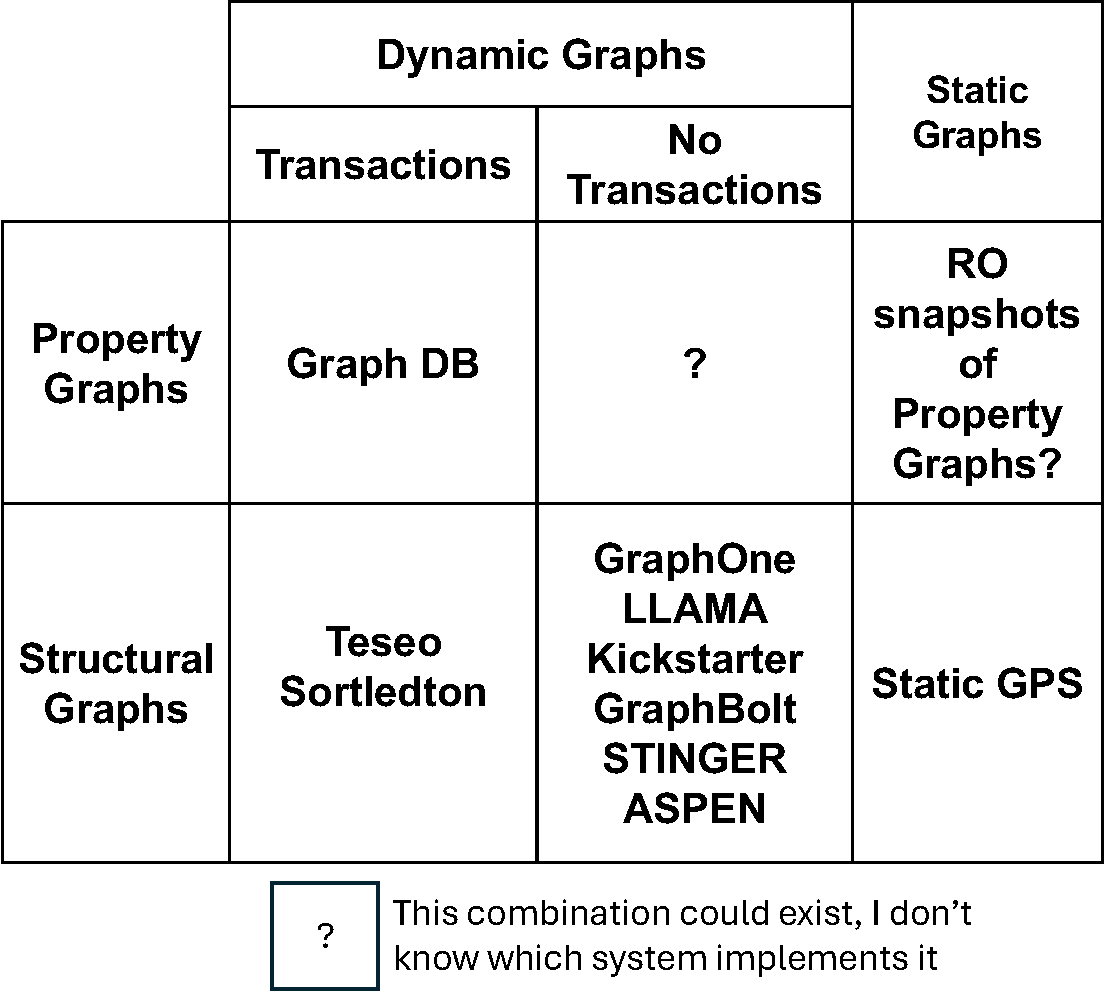
\includegraphics[scale=0.45]{fig/background/design_grid.pdf}
  \caption{Distillation of the design space of graph data management systems. Please refer to Section~\autoref{design:dynamic_structural} for an explanation of how the systems listed in the dynamic but not transactional category differ from one another.}
    \label{fig:distilled_design_space}
\end{figure*}
The main takeaway from this grid is that graph databases are the most general class of graph data management systems: they manage property graphs (of which structural graphs are a subset), support dynamic mutations, and provide transactional guarantees.
All the other categories are specialized to handle a subset of these features.
Each of those systems works well for the use cases for which it was designed, but none is as general as a graph database.
FlexoGraph is designed to be a general-purpose graph data management system that can flexibly support all the specialized use cases depicted in this grid \emph{without having to move the data} or sacrificing performance.
